\documentclass[12pt,a4paper]{article}
\usepackage{times}
\usepackage{durhampaper}
\usepackage{harvard}
\usepackage{listings}
\usepackage[pdftex]{graphicx}
\usepackage{float}

\citationmode{abbr}
\bibliographystyle{agsm}

\title{Analysis of Web Application Vulnerability Detection Algorithms}
\author{David Budgen}
\student{A.J.C. Taylor}
\supervisor{W.W. Song}
\degree{BSc Software Engineering}

\date{}

\begin{document}

\maketitle

\begin{abstract}
    
    {\bf Background}
    The rapid development life-cycle of web applications, encouraged by frameworks such as Ruby on Rails, leaves little time for security testing.  As a result security is often over looked in many web applications that are not security critical.

    Consequently, security vulnerabilities of various severity are prevalent in many web applications.  Manually enumerating every possible area of vulnerability in a web application is a time consuming activity and this is where automated vulnerability detection tools can be of benefit.
    
    {\bf Aims:}
    The aim of this project is to develop and evaluate algorithms to automatically detect vulnerabilities in web applications.  Secondly, a web based tool, will be created to demonstrate the algorithms in action and the real-world potential of the algorithms.
    
    {\bf Method:}
    Use the dynamic scripting language Perl, to prototype and tweak vulnerability detection algorithms, and create a web-based interface and proof-of-concept tool, demonstrating the algorithms.
    
    {\bf Results:}
    Results indicate that the algorithms developed are somewhat successful at automatically detecting vulnerabilities in web applications.  Furthermore, the tool developed adequately demonstrates the algorithms, while being usable and achieving secondary goals of scalability and performance.
    
    {\bf Conclusions:}
    Project Norris (the tool developed) works well, and the results show the relative success of the algorithms developed.  Subsequent work could be done to further develop and improve the algorithms now that a solid foundation is in place.
\end{abstract}

\begin{keywords}
    web application security, sql injection, cross site scripting, xss, brute force, fuzzing
\end{keywords}

\section{Introduction}
The aim of the project is to create and analyse web application vulnerability detection algorithms.  To support the evaluation and analysis of the algorithms, a proof-of-concept web-based tool will be developed that utilises the algorithms to detect vulnerabilities in web applications.

Hypothetically, if the tool were fully complete, the purpose of the tool would be to help security researchers and website owners to identify areas of their websites and web applications that are vulnerable to particular attacks so that they can mitigate the problem(s).

The motivation for the development of such a tool is the fact that it is prohibitively expensive to perform a manual vulnerability analysis of a web application, however, an automated tool can rapidly analyse a web application using several different attack methodologies much faster than a human.

The Open Web Application Security Project (OWASP) maintain an annual list of the most prevalent vulnerabilities found in web applications. \cite{OWASP:2007:Online} The two vulnerabilities the algorithms and tool will be primarily addressing are Cross Site Scripting (XSS) and Injection Flaws, particularly SQL Injection (SQLi) flaws in our work.

Almost half of all the vulnerabilities found in web applications were either XSS vulnerabilities or Injection Flaws, which is why these two vulnerabilities are the primary focus of this research. \cite{OWASP:2007:Online}

XSS vulnerabilities ``allows an attacker to manipulate parts of a Web page... By injecting malicious scripting code" \cite{Holz2006} which according to a report by CERT allows an attacker to ``run malicious code in a users browser with the privileges of a legitimate script originating from the legitimate web server". \cite{Rafail:2001:Online}

Vulnerabilities from XSS attacks include stealing the user's cookies and hijacking their session and/or account, connecting users to malicious servers of the attacker's choice or performing other malicious operations on the user's machine under the guise of the vulnerable site. \cite{Lee:2002:Online}

SQL injection attacks revolve around the attacker ``trying to exploit the data provider at the backend...leading to information disclosure". \cite{Holz2006}

SQL injection attacks “allow attackers to create, read, update, or delete any arbitrary data available to the application. In the worst case scenario, these flaws allow an attacker to completely compromise the application and the underlying systems, even bypassing deeply nested firewalled environments.” \cite{OWASP:2007:Online} 

\section{Related Work}
There are a number of different approaches to vulnerability discovery and prevention.  Some of the discovery work involves static analysis of source code (white box) and some of the prevention work involves input filtering techniques that can be applied to web applications.
Much of the automated vulnerability discovery work has been done by commercial companies, however, there are some free and/or open source implementations.

\subsection{Static Analysis}
Static analysis is a white box technique used to analyse source code for vulnerabilities.  The main limitation of static analysis tools is that they have to be rewritten for every different programming language and/or framework a web application can be written in, and so far, most of the work seems to have focussed only on PHP.  Furthermore, often they struggle to analyse dynamically included content, meaning the PHP analysis is incomplete.

Wasserman and Su worked on static analysis to detect XSS vulnerabilities using a mixture of tainted information flow and  string analysis and were able to provide effective checking algorithms. \cite{Wassermann2008}

Wasserman and Su also worked on a static analysis tool to detect SQLi vulnerabilities.  They constructed a grammar based algorithm which tracks the effects of string operations and checks query construction to see whether users can directly or indirectly influence the query construction.   They then check if the users’ input is sufficiently  isolated from the query construction that it avoids SQLi vulnerabilities. \cite{Wassermann2007}

Jovanovic, Kruegel and  Kirda created an open source tool - Pixy - for static analysis of PHP applications to detect XSS vulnerabilities.  The tool used a “flow sensitive, interprocedural, and context sensitive analysis for PHP” to detect vulnerabilities. \cite{Jovanovic2006}  Pixy is hampered by its inability to scan included PHP files, leading to the authors admitting a number of false-positives being returned by the tool.  Also Pixy does not deal with the object-orientated features of PHP, instead they assume that object member variables are safe, which may not be the case.

Huang et al. created a “lattice-based static analysis algorithm, derived from type systems and typestate”.  They also created a tool - WebSSARI - to analyse PHP source code for XSS and SQLi vulnerabilities. \cite{Huang2004}

\subsection{Input Filtering}
Input filtering research has been undertaken by developing intermediary proxies that can filter out data before it reaches, for example, a user or a database.

Liu et al. developed  a proxy-tool, called SQLProb, to prevent SQLi attacks.  SQLProb sits between the front-end web servers and the back-end databases and uses genetic algorithms to dynamically detect SQLi attacks and block them from reaching the databases. \cite{Liu2009}

SQLProb works in a similar manner to a web application firewall (WAF) and is quite a useful additional layer of security for a web application.  There are a number of other open-source WAFs such as: mod\_security for the Apache web server \cite{ModSecurity:2010:Online} and WebKnight for the IIS web server. \cite{WebKnight:2010:Online}  There are also many commercial WAFs available.

Kirda et al. developed a proxy tool - Noxes - for end-users to sit between  web applications and the users’ browser to mitigate the effect of XSS vulnerabilities on end-users.  Noxes can be thought of as a personal web firewall for end-users. \cite{Kirda2006} Noxes is similar to the FireFox plugin NoScript \cite{NoScript:2010:Online} and suffers the same limitations in that it is extremely invasive to have to block or allow every single request from every new URI.  Noxes plays no role in discovering vulnerabilities in web applications, it is purely for protecting end users.

\subsection{Automated Black Box Vulnerability Discovery}
Automated black box vulnerability discovery tools look at a web application from a [malicious] user’s perspective, i.e. there is no source code analysis involved, and only look at the front-end of the web application.  Much of the research, and the tools developed, has been undertaken by commercial organisations.

WhiteHatSecurity have a commercial scanning tool named Sentinal \cite{WhiteHatSecurity:2010:Online}, HP have WebInspect, a commercial scanning tool \cite{HPWebInspect:2010:Online} and IBM have the Rational AppScan suite of commercial scanning tools \cite{IBM:2010:Online}. 

An open-source automated tool was prototyped by the Secure Systems Lab at the Technical University of Vienna - SecuBat, consisting of a multi-threaded crawling, attack and analysis components.   

By crawling 25,064 pages they were able to ascertain that 6.63\% were vulnerable to SQL Injection attacks and that 5.14\% were vulnerable to XSS attacks. \cite{Kals2006}

Other semi-automated web application scanning tools include CAL9000 \cite{Loomis:2009:Online} a browser based web application security toolkit developed by OWASP to improve certain areas of web application testing procedures. \cite{Grossman2007}

Nikto is another tool which automatically looks for pre-defined vulnerabilities in specific web applications, including XSS and SQL Injection but is unable to automatically detect unknown vulnerabilities or to look for general classes of vulnerabilities. \cite{Nikto:2009:Online} 

Nessus is a similar tool to Nikito and again can find pre-defined vulnerabilities but not general classes of vulnerabilities. \cite{Nessus:2010:Online}

Nikto and Nessus are good at finding specific exploits that have already been exposed, for example a specific SQLi vulnerability in a specific version of an open source blogging platform but neither are capable of automatically detecting XSS or SQLi vulnerabilities in general.

\subsection{Summary}
As can be seen from the literature the current emphasis of academic research into web application vulnerability detection centres around static analysis of web application code bases.

This is impractical because web applications can be written in many different languages, using many different frameworks whereas the literature survey uncovers only PHP static analysis tools.  Furthermore, the literature clearly states that these tools are incomplete due to the dynamic nature of the PHP language and the ability to dynamically include code at run-time.

On the other hand, tools based on the idea of black box vulnerability scanning can be used on web applications implemented in any language because they pay no attention to the source code of the application.

Consequently, the research and development of a black box, automated vulnerability scanning tool appears to be the best direction to take to ensure maximum web application coverage.  It is hoped that this ability to analyse web applications written in any language will be a large improvement over other static analysis tools.

\section{Solution}

\subsection{Architecture and Design}

\subsubsection{Overview}
Figure~\ref{fig:overview} provides an architectural overview of Project Norris, the proposed solution.

\begin{figure}[!ht]
    \begin{center}
        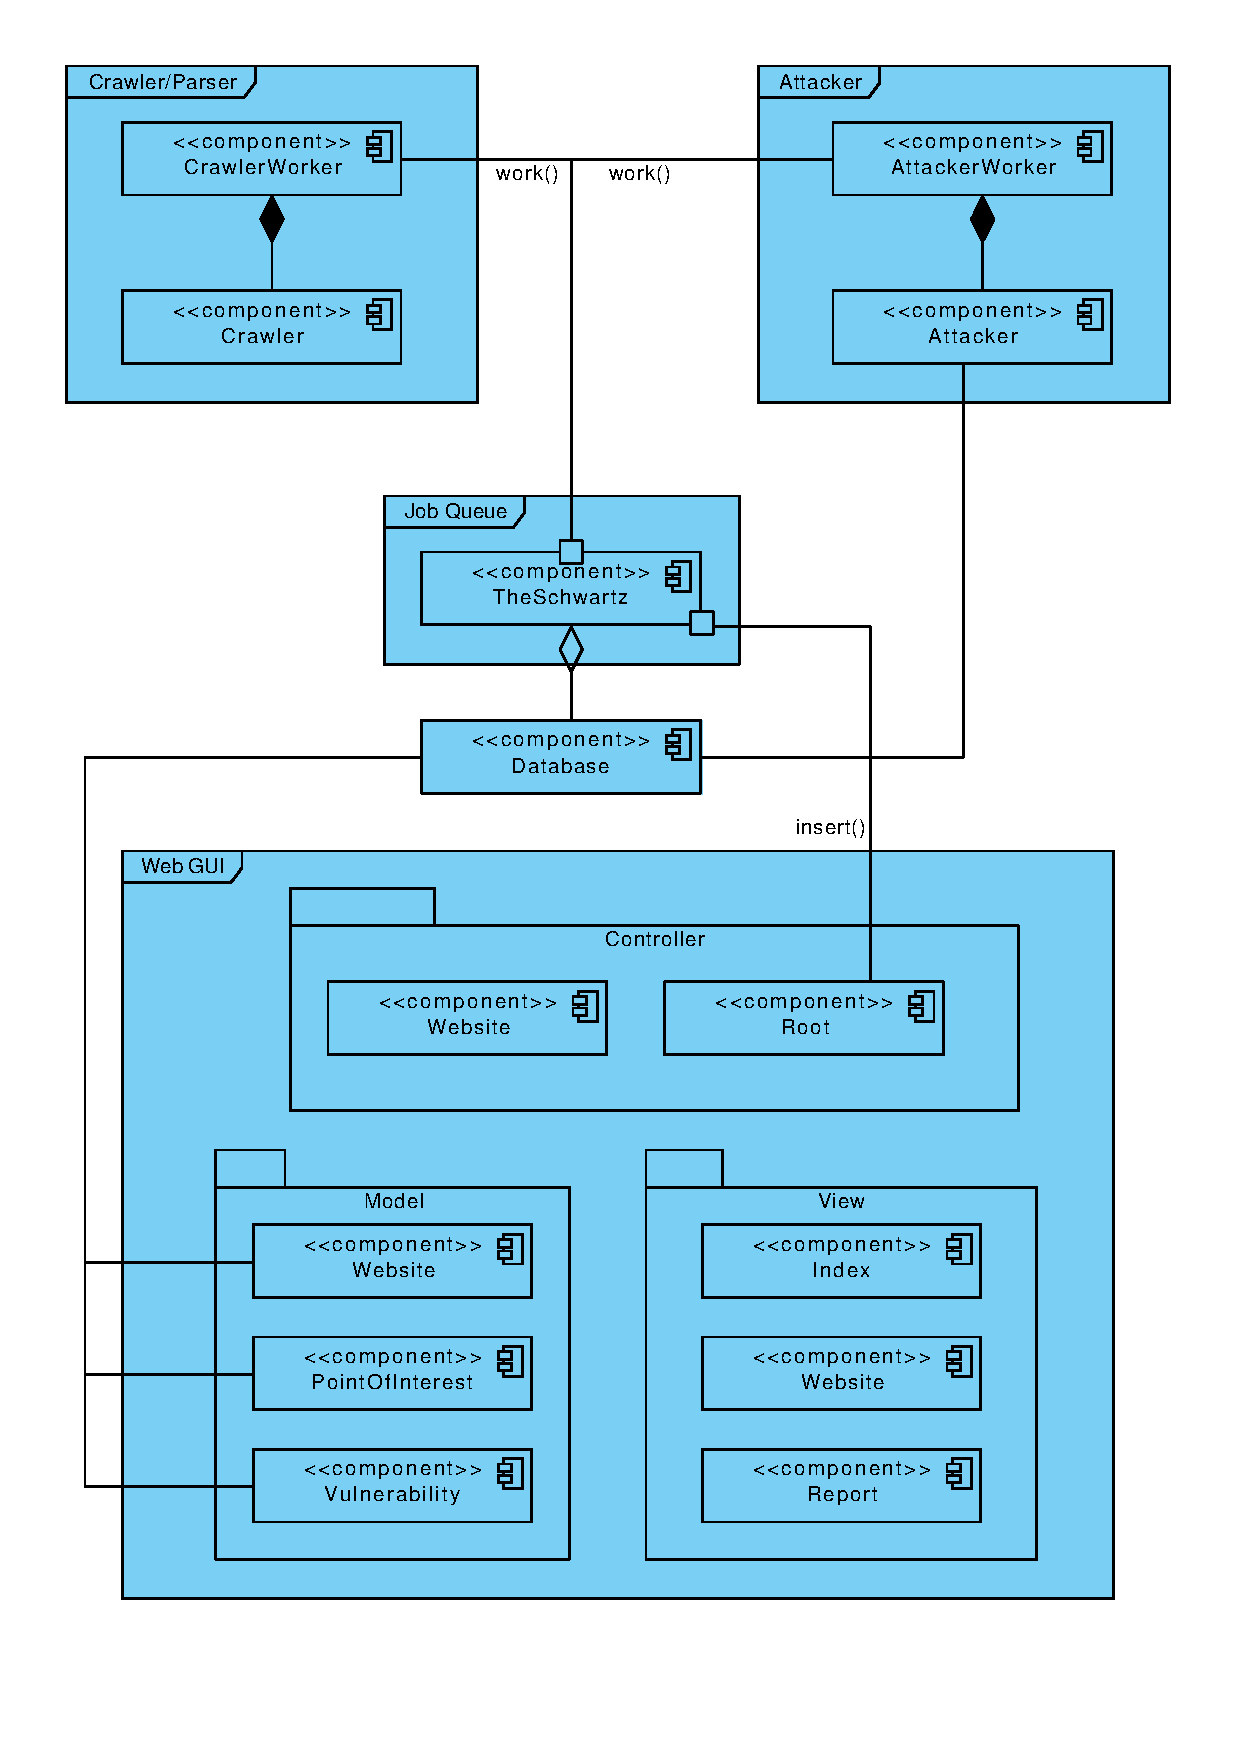
\includegraphics[scale=0.5]{images/overview_component_diagram.pdf}    
    \end{center}
    \caption{Component Diagram of Project Norris}
    \label{fig:overview}
\end{figure}

Project Norris is a web-based application that allows a user to input a URL of a website, and then after crawling, parsing, and attacking the website, displays a report to the user of any security vulnerabilities found in the website by Project Norris.

The design of Project Norris has been broken down into a number of core components.  The user interface of Project Norris is handled by an model-view-controller (MVC) based web application.  There are then two main back-end components which do the heavy processing for the application.  These are the Attacker component and the Crawler component.

The Web GUI interacts with the back-end components by placing jobs on another component, the Queue.

The Attacker and Crawler are further broken down into two components each, one being a worker script which is continuously run that checks for new jobs on the Queue and the other component being the code that is run by the script when a job is found.

Many of the components also rely on another component, the Database. This is to allow data to be stored persistently rather than only in-memory, i.e. all the data related to vulnerabilities found in web applications are stored in the database.

The Queue component relies heavily on the Database because when a job is added to the Queue it is actually inserted into the Database.  Consequently when the two worker scripts are asking the Queue if there are any available jobs, the Queue actually just queries the database.

The reason to separate the back-end from the front-end of the web application is to deal with the issue of cohesion and coupling, and performance and scalability.  %TODO refs / further explanation

\subsubsection{Web GUI}
The Web GUI, or the front-end of the Project Norris web application, is designed using the MVC architectural pattern.

The various different views of the Web GUI are displayed to the users by the controllers retrieving any required data from any relevant models and then loading the relevant view and passing the data.

Views are simply template files, possibly with place holders for data and simple logic for dynamic code, rendered inside a global template file, with data being passed in via controllers.

\subsubsection{Queue}
The Queue is simply a `first in first out', database-backed job allocation system.  It works in the following way:

A job is inserted into the Queue (and hence the database) containing, among other things, a reference to the function of work this particular job is associated with and any arguments the job requires.

For example, to add a new website to be crawled, a job is added to the queue containing a reference to the fact that it is a crawling job and the arguments passed are the url of the website.

Worker scripts are started, and left continuously running, that poll the queue at set intervals looking for work they can perform.  If they find any work, they dequeue the job and then using the module with the actual job functionality implemented they perform the task and then go back to looking at the queue until another job appears which they can perform.

The activity diagram, Figure ~\ref{fig:queue}, represents this process.

\begin{figure}[!ht]
    \begin{center}
        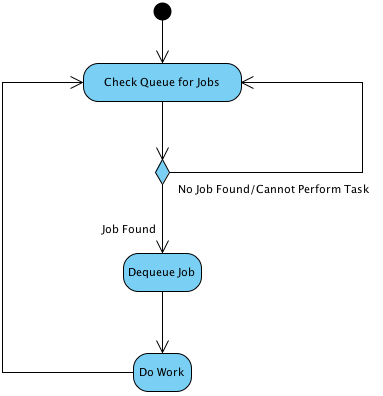
\includegraphics[scale=0.7]{images/queue_activity_diagram.png}    
    \end{center}
    \caption{Activity Diagram of Project Norris' Queue}
    \label{fig:queue}
\end{figure}

\subsubsection{Database}
The Database is an integral component in allowing persistent storage of data and is crucial to the function of the Queue. 

The models in the Web GUI are backed by tables in the database, with an object-relational mapper (ORM) layer between, allowing objects in the Web GUI to be persistently stored beyond one HTTP request.

There are three main tables used throughout the application:

\begin{itemize}
    \item{Websites - A website is a URL which a user enters to be scanned.}
    \item{PointsOfInterest - A PointOfInterest is any forms, or URL fragments that the crawler/parser finds when crawling the Website.  These are what are passed to the Attacker to look for vulnerabilities...}
    \item{Vulnerabilities - Any vulnerabilities found by the attacker are stored in the Vulnerability table.}
\end{itemize}

In essence, a Website has many PointsOfInterest and each PointOfInterest can have many Vulnerabilities.

\subsubsection{Crawler/Parser}
The crawler has been designed to use a Breadth First Search algorithm.  It is passed a base URL and it then finds all the links on that page and adds them to a queue.  It then proceeds to dequeue one URL at a time and and get all the links on that page and then put them on its queue (unless any of them have already been visited - it maintains a hash so it can quickly check whether or not a URL has been seen before).

The pages are parsed using regular expressions.  As well as looking for links it also looks for forms, which can be parsed to the Attacker.  Forms have been chosen as it is the obvious place where a [malicious] user can submit input to the application.  The URI of the page is also checked to see whether it contains a query string, if so, this is also added to the Queue for the Attacker as it suggests the possibility of a file inclusion/directory traversal vulnerability.

The activity diagram, Figure \ref{fig:crawler}, shows how the crawler works.

\begin{figure}[!ht]
    \begin{center}
        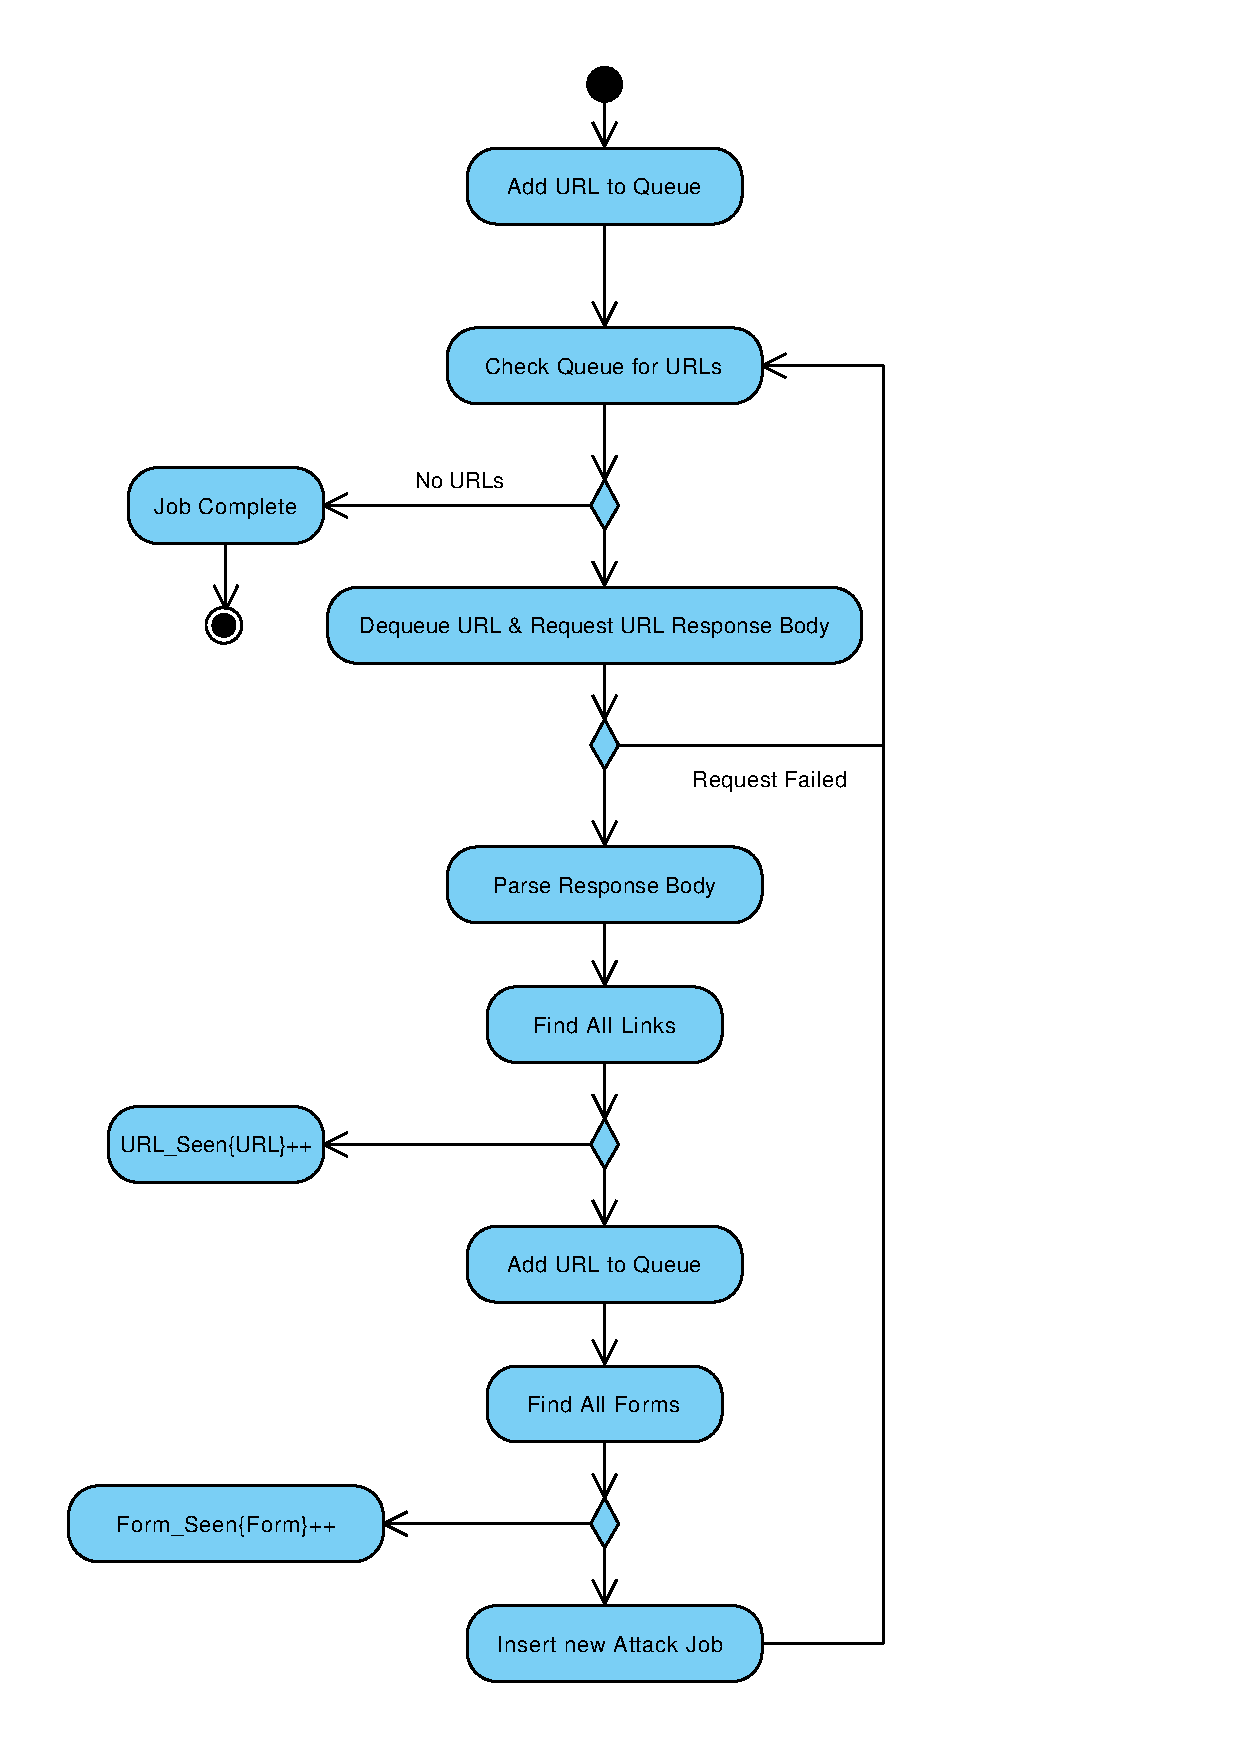
\includegraphics[scale=0.5]{images/crawler_activity_diagram.pdf}    
    \end{center}
    \caption{Activity Diagram of Project Norris' Crawler}
    \label{fig:crawler}
\end{figure}

\subsubsection{Attacker}
The attacking component receives a job from the Queue with an object representing a PointOfInterest (found by the Crawler), and then proceeds to input different attack vectors, submit the form (or request the new URI) and parse the HTTP Response Body or Header, sent from the server, to see whether or not the attack was successful.

The attacking component is also responsible for storing data.  Every time it starts a job it adds information about the job into the database so in the GUI every point of possible vulnerability (PointOfInterest) is reportable. 

For any successful attacks a vulnerability is stored which is associated with a specific PointOfInterest (which is in turn associated with a Website).

\subsubsection{Workflow}
The workflow between the various components is demonstrated in the sequence diagram (Figure ~\ref{fig:workflow}).

\begin{figure}[!ht]
    \begin{center}
        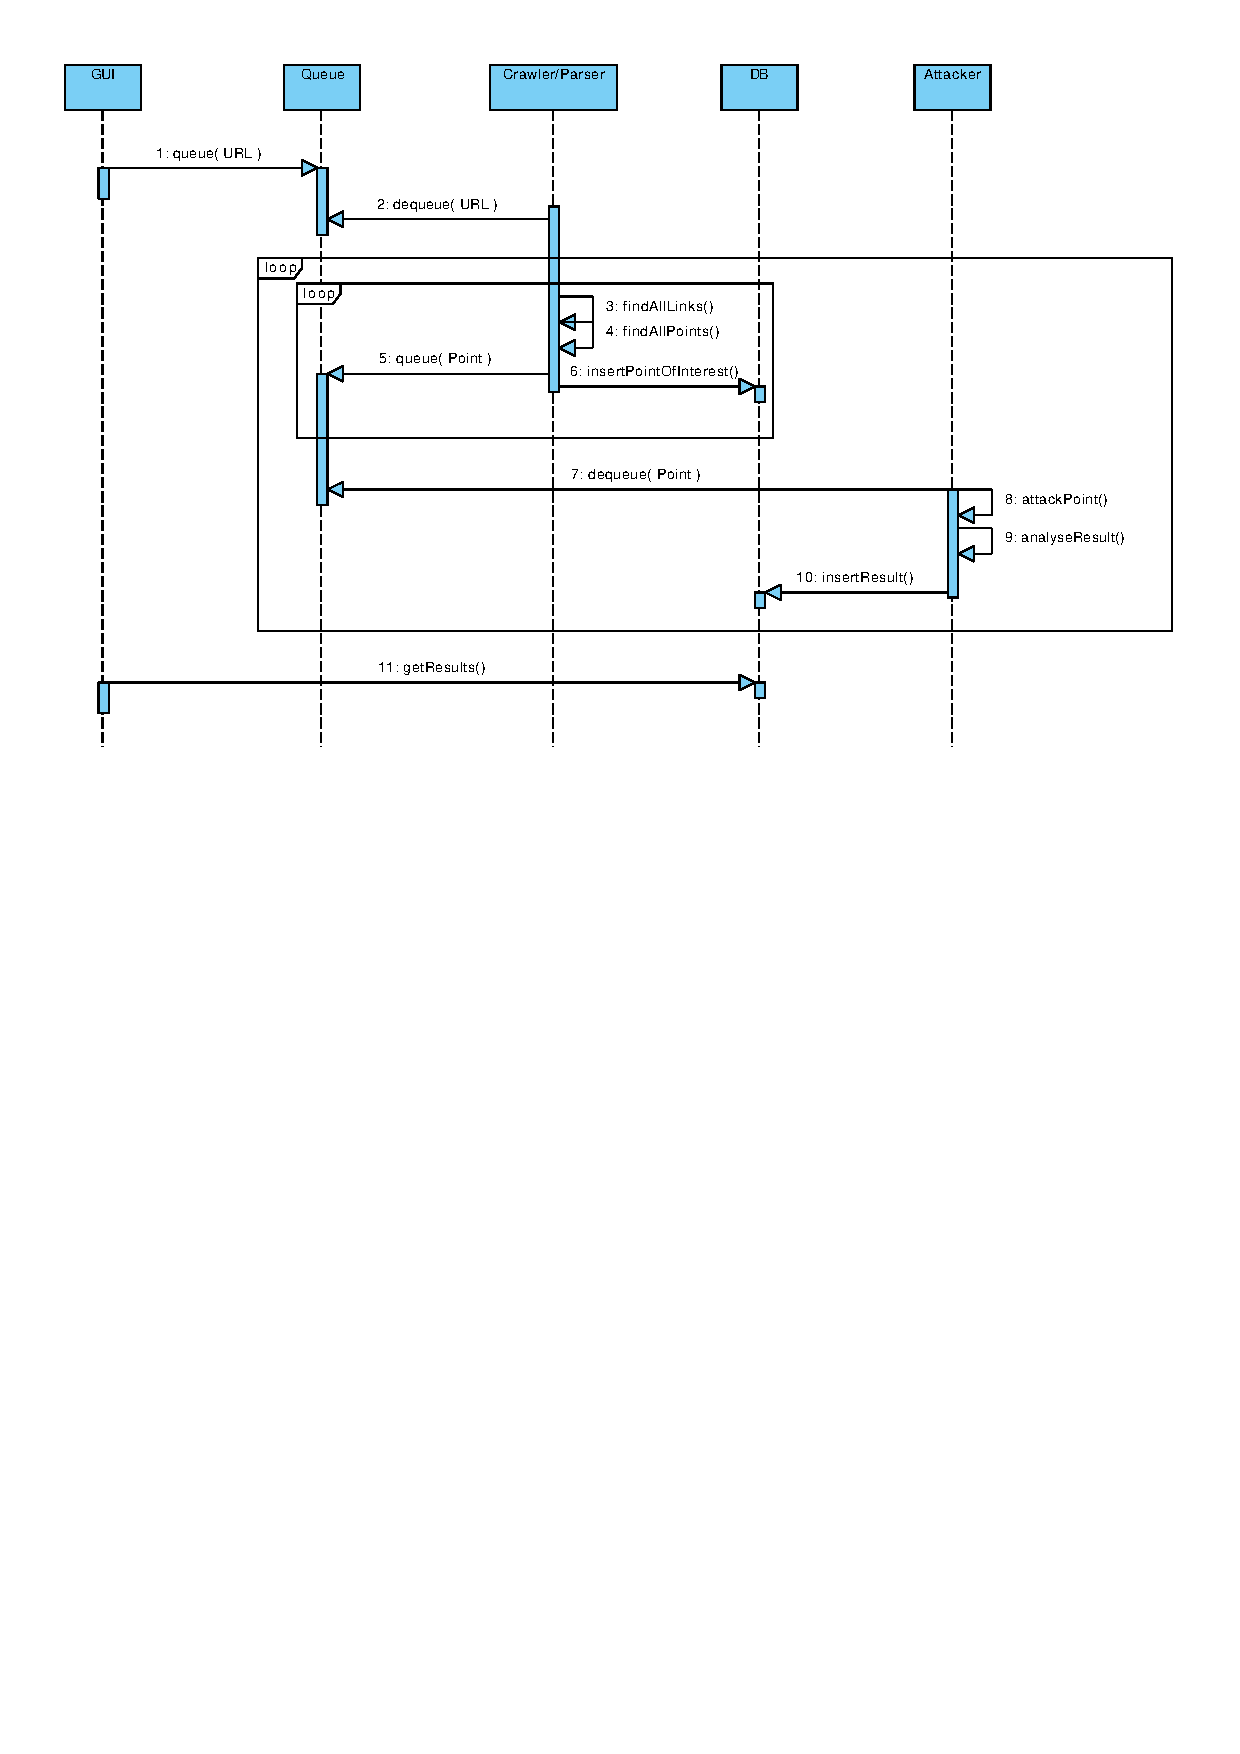
\includegraphics[angle=90]{images/system_sequence_diagram.pdf}    
    \end{center}
    \caption{Sequence Diagram of Project Norris}
    \label{fig:workflow}
\end{figure}

% TODO this following section is a bit repeated

When a user first visits Project Norris in a web browser, they are presented with an opportunity to add a URL to the system.  This then allows them to scan the URL/domain and later, view reports of vulnerabilities found.  If they choose to scan the URL the Web GUI then places the URL onto the Queue.

There are two worker scripts, one for the Crawler/Parser and one for the Attacker, which are continually polling the Queue for jobs.

As soon as the Crawler sees that there is a job available (i.e. the URL just placed onto the Queue by the Web GUI) a cycle kicks in where the Crawler takes the URL and crawls the whole site finding every page on the domain.  It maintains it’s own internal queue of the URLs on the domain, to ensure it only processes new URLs.

It enters a loop where it enqueues every unseen link on a page into the queue and looks for any PointsOfInterest (i.e. forms or URIs that contain a query string) on the page, which if it finds, inserts as a job on the Queue for the Attacker, then it dequeues the next URL to look at until there are no more pages on the domain to crawl.

When it has finished crawling and parsing the whole website it goes back to watching the Queue for new jobs.

The attacker takes a form off the Queue and then proceeds to attack the form and analyse the response from the web server.  Should a vulnerability be detected, it is then inserted into the database for the Web GUI to generate reports to the user.  It's also important to note that the Attacker starts working \emph{as soon as} the Crawler/Parser finds a PointOfInterest and adds it to the Queue.  This allows for asynchronous crawling/attacking which helps to speed up the vulnerability discovery process.

The user is then able to generate reports in the Web GUI, which are created using the data in the database collected by the Attacker.

\subsubsection{Data Flow}
Data flows through Project Norris in the way illustrated in Figure ~\ref{fig:dataflow}.

\begin{figure}[!ht]
    \begin{center}
        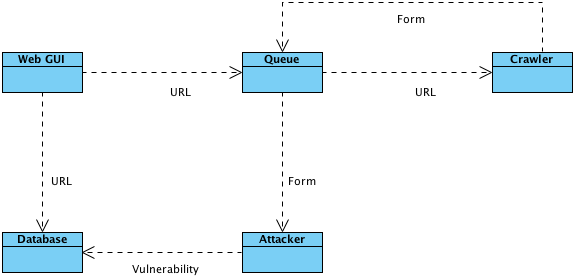
\includegraphics[scale=0.7]{images/data_flow_diagram.png}    
    \end{center}
    \caption{Data Flow Diagram of Project Norris}
    \label{fig:dataflow}
\end{figure}

\begin{itemize}
    \item A URL is inserted into the Queue and a Website object is created and stored in the database
    \item The Crawler dequeues the URL and proceeds to crawl and parse the whole domain.  Any PointsOfInterest it finds are inserted into the Queue.
    \item The Attacker dequeues any PointsOfInterest in the Queue and proceeds to attack the PointOfInterest.  The PointsOfInterest themselves are inserted into the database by creating PointOfInterest objects and any successful attacks are stored as Vulnerability objects in the database.
\end{itemize}

So one Website can have many PointsOfInterest, and one PointOfInterest can have many Vulnerabilities.

\subsubsection{Limitations}
Project Norris is a web application and this may limit it’s usefulness to the average end user, having said that, it has been written as a “hosted solution”.

Project Norris also suffers a limitation of not looking at every aspect of a website that may be vulnerable.  The focus is primarily on input forms, whereas cookies and query strings may also contain vulnerabilities.

The detection of SQL Injection attacks is also limited by the fact that different web and SQL servers throw different errors on receipt of invalid SQL statements.  This means that the Attacker will have to be “trained” to understand what types of responses likely indicate an SQL Injection vulnerability, however this is likely to be imperfect.

\section{Implementation}
The general procedure for processing a URL is as follows:

\begin{itemize}
    \item A user adds a Website to the system.
    \item A user chooses to scan a particular Website for vulnerabilities.
    \item The URL of the Website is placed onto the Queue by the GUI.
    \item The Crawler sees the URL on the Queue and dequeues the job.
    \item The Crawler establishes its own queue of urls, starting with the URL from in the job.
    \item The Crawler then proceeds to parse the page finding every link (and maintains another data structure, a hash, to check for unique URLs) and adds them to its internal queue.
    \item The Crawler also looks for any PointsOfInterest on the page and if it finds any adds it to the Queue as a job for the Attacker.
    \item The Crawler then dequeues the next URL from its internal queue and continues through this loop until there are no URLs left on the queue to process.
    \item When the Attacker dequeues a job, it first inserts the PointOfInterest into the Database.
    \item The Attacker then runs through the various vulnerability detection algorithms and if it finds any vulnerabilities it stores them in the Database.
    \item The user is then free to generate a report for any previously scanned websites in the GUI.  These reports are generated dynamically via data stored in the Database by the Attacker.
\end{itemize}

\subsection{Algorithms}
There are two vulnerability detection algorithms in Project Norris.  Both are fairly primitive and follow a similar work flow:

For a given form: send malicious data, analyse the server response or the HTTP Response Body of the generated page, and the HTTP Header, to ascertain whether the attack was successful.

The difference between the two algorithms is the method of generating the malicious data to send.

\subsubsection{Static Brute Forcing}
Static Brute Forcing will take a list of known attack vectors, and permeate through the list until one succeeds or none of the attacks succeed.  The list of attack vectors will be generated from the XSS Cheat Sheet \cite{Hansen:2009:Online}.

The pseudo-code for the algorithm is along the following lines:

\begin{lstlisting}
def StaticBruteForce( PointOfInterest )     
    <List> vectors;
    
    foreach (vector in vectors) { 
        attackPoint( vector );
    }
end
\end{lstlisting}

This algorithm is primarily used for detecting XSS vulnerabilities but an even simpler version that inputs only one single-quote - ' - will be used to detect SQLi vulnerabilities.

\subsubsection{Fuzzy Brute Forcing}
Fuzzy Brute Forcing dynamically generates potentially malicious input by generating a large amount of random data. \cite{Sutton2007}

The pseudo-code for the algorithm is along the following lines:

\begin{lstlisting} 
def FuzzyBruteForce( PointOfInterest )
	for (1..1000) {
		
	    attackPoint( fuzzyVector() );
	
	}
end
\end{lstlisting}
This algorithm will be used to look at a different vulnerability: directory traversal vulnerabilities. Directory traversal vulnerabilities are where it is possible to display files on the server, in the browser that are outside of the normal web application files.  For example, one way of displaying pages is to pass a file name to a script, which then loads the file.  By passing a specially crafted file name, it may be possible to display files that are not intended for viewing (such as system or password files). % TODO reference

\subsection{Web GUI Implementation}
The GUI is a simple web application that allows a user to add or delete websites, to initiate a new scan of a website (which means to place the URL onto the job queue for the crawler and attacker) and to view reports.  A screenshot can be seen in Figure ~\ref{fig:gui}.

\begin{figure}[!ht]
    \begin{center}
        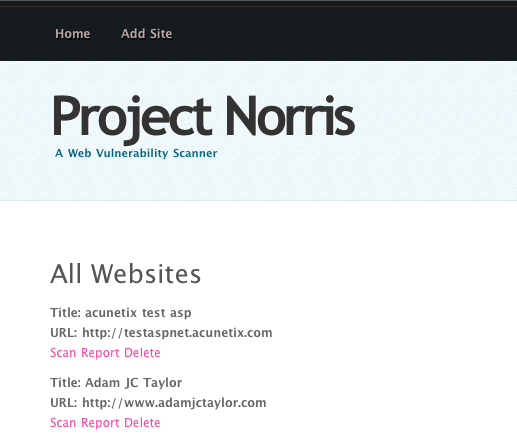
\includegraphics[scale=0.7]{images/gui.png}    
    \end{center}
    \caption{GUI Screenshot}
    \label{fig:gui}
\end{figure}

% TODO reference perl modules

The GUI has been developed using the Catalyst web framework.  Catalyst is a Perl model-view-controller (MVC) based framework.  It provides helpers for many common tasks in web application development, provides architectural guidance yet still allows for flexibility to develop the application as desired.

DBIx::Class is a Perl object relational mapper (ORM).  It is used to map objects created in the GUI directly to rows in the database.  It provides a clean interface for constructing SQL queries and persistently storing objects and has been used alongside Catalyst in the development of the GUI.

The reports are generated dynamically from data in the Database and use the JavaScript HighCharts API to improve the visualisation of the results as seen in Figure ~\ref{fig:report}.

\begin{figure}[!ht]
    \begin{center}
        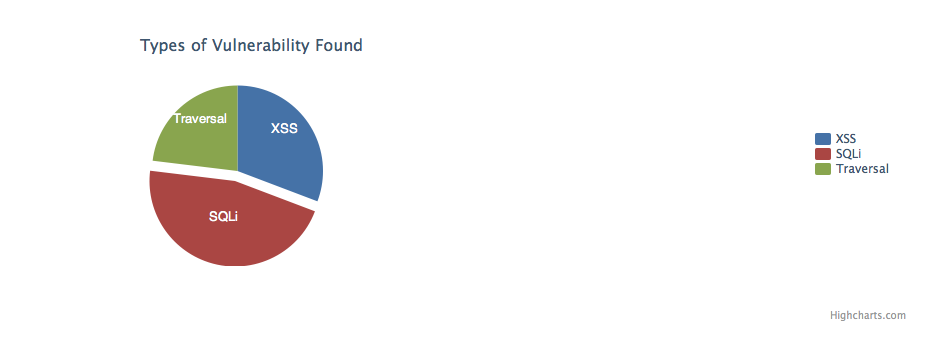
\includegraphics[scale=0.7]{images/report.png}    
    \end{center}
    \caption{Report Visualisation in GUI}
    \label{fig:report}
\end{figure}

\subsection{Job Queue}
The Job Queue is used to pass jobs between the GUI, the Crawler and the Attacker.  Without the Job Queue this whole communication process would be tightly coupled and, save multi-threading, would cause the GUI to lock up while components finished their tasks.

The Queue is implemented using a Perl module called TheSchwartz, which uses the Database for storing specific jobs as well as meta data about which components can perform which tasks.

The Crawler and the Attacker and then started up and continuously poll the database/queue looking for new jobs which they can perform, once they are complete they then look for more jobs.

\subsection{Crawler}
The Crawler receives a URL from the GUI in the job it receives from the Queue.  It then initialises a queue of its own with the initial URL on and enters a while loop, whose precondition is that the queue has at least one item on it.  The Crawler then proceeds to find every link on that page using the Perl module WWW::Mechanize.  As well as the queue it maintains a hash of \{ URL =$>$ no. of times seen \}.  For each link it finds on each page it checks whether or not it exists in the hash, if not it adds that link to the queue and if so it simply increments the count of the number of times it has been seen.

It also performs some additional checks before following a URL: it makes sure that it only follows links to pages that are of content type `text/html',  it only follows URLs of pages on the same top level domain (TLD) as the initial URL and it treats http://example.com/about and http://example.com/about\#careers as the same URL to avoid excessively crawling the same page.

While on a page it also looks for PointsOfInterest that can be passed to the Attacker.  If it finds a form on the page, it inserts a new job on the Queue with a reference to the form it found for the Attacker to perform XSS and SQLi attacks.  If it finds a URI with a query string, such as, http://example.com/index.php?page=../home.php, it inserts a new job on the Queue with a reference to the URI for the Attacker to perform a directory traversal attack and a SQLi attack.

\subsection{Attacker}
The Attacker component first checks to see whether it has received a URI or a Form PointOfInterest and stores the PointOfInterest in the Database for the GUI.  If it is a URI PointOfInterest it executes the directory traversal, fuzzy-based algorithm.  This works by attempting to access $<$\$input\_uri$>$../etc/passwd, then $<$\$input\_uri$>$../../etc/passwd and so on and looking, via regular expression, for the word `root' (as in the root user accout) in the HTTP Response Body returned from the server.  If it is found a Vulnerability is stored in the database for that particular PointOfInterest.  It also, tries the SQLi algorithm, explained shortly.

This can return false positives and only works on unix based servers.

If it has been passed a Form PointofInterest from the Crawler it first executes the XSS algorithm and then the SQLi algorithm.  The XSS algorithm works by permeating through a list of predefined attack vectors. For each iteration through the list of vectors, the vector is set as the input for each field of the form, which is then submitted, and in the HTTP Response Body the attack vector is searched for, via regular expressions.  If it is found then it is assumed that the vector was successful and a Vulnerability is stored in the database for that PointOfInterest.

The SQLi injection algorithm works by inserting a single quote - ' - into all the input fields and attempts to work out if a server or database error was thrown in response.  This is done by checking the HTTP Response Header from the server to check whether or not it is in the 50x range - indicating an error - or looking for common database error phrases output by different database systems in the HTTP Response Body.  

This is incomplete as sometimes false positives are found if certain phrases assumed to demonstrate SQLi vulnerabilities are present in the HTTP Response Body and also we do not have a full list of all the errors sent by all different types and versions of database systems.

\subsection{Database}
The database (MySQL 5) for storing data related to a website contains three primary tables:

A \emph{Website} contains a name and URL.
A \emph{Website} has many \emph{PointsOfInterest} where a point of interest is a URL.
A \emph{PointOfInterest} has many \emph{Vulnerabilities} where a \emph{Vulnerability} has a type and an input string.

Two intermediary tables are used to normalise the many-to-many relationships: \emph{WebsitePointOfInterest} and \emph{PointOfInterestVulnerability}.

The specific table structures are as follows:

websites\{ id, url, name \}

points\_of\_interest\{ id, url \}

vulnerabilities\{ id, type, input \}

website\_point\_of\_interest\{ website\_id, point\_of\_interest\_id \}

point\_of\_interest\_vulnerability\{ point\_of\_interest\_id, vulnerability\_id \}

The queries are generated using the module DBIx::Class which maps objects to rows in the database.  It allows query construction in the GUI as follows:

\begin{lstlisting}{language=Perl}
    $website->find($id)->points_of_interest();
\end{lstlisting}

\subsection{Testing}
The project has a number of system tests, implemented using the Test::More module which uses the Test Anything Protocol (TAP) to output simple text-based results.  This provides a means of ensuring the various front-end facing features of the tool are working as expected.

\section{Results}

\subsection{Primary Results}
The primary results where taking against a scan of the Damn Vulnerable Web Application (DVWA) an open source, PHP web application for security research and learning. \cite{DVWA:2010:Online}

\begin{center}
    \begin{table}
        \caption{DVWA Scan Results}
        \begin{center}
            \begin{tabular}{ | l | r | }
                \hline
                Vulns Found & 4 \\ \hline
                \% Found & 100 \\ \hline
                Vulns Missed & 0 \\ \hline
                \% Missed & 0 \\ \hline
                False Positives & 3 \\ 
                \hline
            \end{tabular}
        \end{center}
    \end{table}
\end{center}

Project Norris reported 7 vulnerabilities found against 10 points of interest.  These were 3 SQLi vulnerabilities, 2 directory traversal vulnerabilities and 2 XSS vulnerabilities.

Of the three SQLi vulnerabilities only one was a real SQLi vulnerability.  The other two were false positives from the liberal nature of trying to detect an SQL error in a page.  It was assumed that the words `sql' and `error' on a page would signify an SQL error.  However, sometimes these were present on random pages in the application.

Of the two directory traversal vulnerabilities only one was a real directory traversal vulnerability.  Again, this was due to the liberal nature of trying to detect when an error occurred.  Directory traversal vulnerabilities are presumed present when `root' is found in the returned page.  This is due to the speculation that the root user is always present in the /etc/passwd file on a unix based system, hence we must have found a vulnerability.

Of the two XSS vulnerabilities found both were real XSS vulnerabilities.  The accuracy of the XSS detection is due to the accuracy in which they are assumed vulnerable.  An XSS vulnerability is only assumed apparent if the exact attack vector is found in the page returned.

This suggests a false positive ratio of 3:7 - we can be just over 50\% sure in the results returned by Project Norris.

It is important to note that while false positives were found, all the vulnerabilities present, that the tool can detect, were also found.

\subsection{Secondary Results}
After testing the tool against DVWA it was then sent out `into the wild' and tested against various security scanner vendor's test web applications.  Again these are deliberately insecure applications, which are a good test of the accuracy of the tool.  An overview of the results is presented followed by more detailed results for each individual application.

The evaluation was based on unpublished research, comparing various commercial scanners, against the various test applications. \cite{Suto2010}

\begin{center}
    \begin{table}
        \caption{Overall Scan Results}
        \begin{center}
            \begin{tabular}{ | l | c | c | c | c | c | }
                \hline
                Site & Vuln Found & \% Found & Vulns Missed & \% Missed & False Positives  \\ \hline
                Acunetix AspNet & 2 & 40 & 3 & 60 & 5 \\ \hline
                Acunetix TestPHP & 3 & 21 & 10 & 79 & 0 \\ \hline
                HP zerowebappsecurity & 2 & 15 & 11 & 85 & 3 \\ \hline
                IBM Testfire & 3 & 20 & 12 & 80 & 1 \\ 
                \hline
            \end{tabular}
        \end{center}
    \end{table}
\end{center}

\begin{center}
    \begin{table}
        \caption{Acunetix AspNet Scan Result}
        \begin{center}
            \begin{tabular}{ | l | c | c | }
                \hline
                Status & Vuln Type & File \\ \hline
                False Positive & SQLi & /ReadNews.aspx?id=0\&NewsAd=ads\%2fdef.html \\ \hline
                False Positive & SQLi & /default.aspx \\ \hline
                False Positive & SQLi & /about.aspx \\ \hline
                Duplicate False Positive & SQLi & /ReadNews.aspx?id=3\&NewsAd=ads\%2fdef.html \\ \hline
                Verified & SQLi & /Comments.aspx?id=2 \\ \hline
                Duplicate False Positive & SQLi & /ReadNews.aspx?id=0\&NewsAd=ads/def.html \\ \hline
                Duplicate False Positive & SQLi & /ReadNews.aspx?id=3 \\ \hline
                Duplicate False Positive & SQLi & /ReadNews.aspx?id=2 \\ \hline
                False Positive & SQLi & /Signup.aspx \\ \hline
                Duplicate False Positive & SQLi & /ReadNews.aspx?id=0 \\ \hline
                Duplicate False Positive & SQLi & /ReadNews.aspx?id=2\&NewsAd=ads\%2fdef.html \\ \hline
                Verified & SQLi & /login.aspx \\ \hline
                Duplicate & SQLi & /Comments.aspx?id=0 \\ \hline
                False Positive & SQLi & /Default.aspx \\ \hline
                Duplicate & SQLi & /Comments.aspx?id=3 \\
                \hline
            \end{tabular}
        \end{center}
    \end{table}
\end{center}

\begin{center}
    \begin{table}
        \caption{Acunetix TestPHP Scan Result}
        \begin{center}
            \begin{tabular}{ | l | c | c | }
                \hline
                Status & Vuln Type & File \\ \hline
                Verified & XSS & /userinfo.php \\ \hline
                Verified & SQLi & /listproducts.php?artist=3 \\ \hline
                Verified & SQLi & /listproducts.php?cat=4 \\ 
                \hline
            \end{tabular}
        \end{center}
    \end{table}
\end{center}

\begin{center}
    \begin{table}
        \caption{HP zerowebappsecurity Scan Result}
        \begin{center}
            \begin{tabular}{ | l | c | c | }
                \hline
                Status & Vuln Type & File \\ \hline
                False Positive & Directory Traversal & /banklogin.asp?serviceName=../etc/passwd \\ \hline
                False Positive & XSS & /pcomboindex.asp \\ \hline
                False Positive & XSS & /login1.asp \\ \hline
                Verified & SQLi & /login1.asp \\ \hline
                Verified & SQLi & /rootlogin.asp \\
                \hline
            \end{tabular}
        \end{center}
    \end{table}
\end{center}

\begin{center}
    \begin{table}
        \caption{IBM Testfire Scan Result}
        \begin{center}
            \begin{tabular}{ | l | c | c | }
                \hline
                Status & Vuln Type & File \\ \hline
                Verified & XSS & /search.aspx \\ \hline
                Verified & XSS & /survey\_complete.aspx \\ \hline
                False Positive & XSS & /bank/login.aspx \\ \hline
                Verified & SQLi & /bank/login.aspx \\ 
                \hline
            \end{tabular}
        \end{center}
    \end{table}
\end{center}

\section{Evaluation}
The primary evaluation of the tool and hence, the algorithms, has been against a slightly modified version of the Damn Vulnerable Web Application.  This is a sample PHP based web application that anyone can freely obtain that has a number of security flaws embedded within.  It is for manual testing and understanding and learning about web application vulnerabilities.  It has been used in this case as a demo application for which to test and evaluate the tool against.

The modifications made were to remove the need to login as at present the Crawler is unable to login and follow pages behind authorisation protection.

\subsection{Comparison}
Comparing my tool to experimental research, it is clear that some of the commercial tools are far superior. It would appear at first glance, that Project Norris is worse than all the other tools tested, and this is true. \cite{Suto2010}

However, some reasons can be given for the relative poor performance in the wild. Regarding XSS vulnerabilities, a common attack vector is:

\begin{lstlisting}
';alert(String.fromCharCode(88,83,83))//
\';alert(String.fromCharCode(88,83,83))//
";alert(String.fromCharCode(88,83,83))//
\";alert(String.fromCharCode(88,83,83))//
--></SCRIPT>">'><SCRIPT>alert(String.fromCharCode(88,83,83))</SCRIPT>
\end{lstlisting}

Regular Expressions have been utilised as the main method of checking whether or not an attack vector was successful. With all the special characters in the attack vector it's proven impossible to match the string in the wild.  Had it been possible, a whole host of extra XSS vulnerabilities could be detected by the algorithm.

The relatively high occurrence of false positives being reported can be explained by the imprecise detection of SQLi and directory traversal vulnerabilities.  Both algorithms `detect' vulnerabilities by looking for certain strings in the output page.  While these strings generally indicate a vulnerability, it's possible it could be present on a page anyway, consequently tricking the algorithm into thinking it has found a vulnerability when it hasn't.  For example, finding `SQL' and `Error' on a page is assumed to indicate an SQL based error message, and hence an SQLi vulnerability but could in fact be present in a page.

Further research into all the possible error strings output by all the various different database engines may lead to a less error prone, and more thorough detection of SQLi vulnerabilities.

Another area of improvement would be to improve the crawler by allowing the user to supply login credentials to crawl and analyse pages behind authentication mechanisms. Furthermore, currently the crawler ignores subdomains and only scans pages directly under the top-level domain (TLD), again it would be useful to be able to crawl these as well.  Also, there are many other types of vulnerabilities that the algorithms fail to address and further work could be undertaken to address a wider range of vulnerabilities.

One strong positive of the tool, compared to other academic research, is the fact that it can be used against web applications of any type, written in any language, and it will do its best to uncover vulnerabilities in that application.  This is possible due to its `black box' nature.

Furthermore, while it currently lags behind commercial tools, one must consider the fact that they are precisely that: commercial tools.  Many of these are state-of-the-art vulnerability detection and analysis tools, developed by commercial organisations, with much larger research and development resources.  With that in mind, Project Norris can be considered as a reasonable first attempt at developing a tool and algorithms.
% TODO more analysis

\subsection{Performance}
The Crawler of Project Norris was timed when crawling web applications of various sizes to see roughly how well it performs.  See Figure ~\ref{fig:performance}.
The sites crawled contained ~100, ~1000 and ~5000 pages respectively.  The time taken to crawl increases with the number of pages crawled.

The pages crawled per second for each site can be seen in Table ~\ref{table:performance}.

\begin{center}
    \begin{table}
        \caption{Crawler Performance}
        \begin{center}
            \begin{tabular}{ | l | c | c | }
                \hline
                \# Pages & Total Crawl Time (s) & Time Per Page (s) \\ \hline
                163 & 196 & 1.20 \\ \hline
                1298 & 1034 & 0.80 \\ \hline
                4945 & 5316 & 0.93 \\ 
                \hline
            \end{tabular}
        \end{center}
        \label{table:performance}
    \end{table}
\end{center}

It's hard to draw any useful conclusions from this data as there are many factors effecting the crawl rate, other than simply the number of pages: network latency and the number of points of interest found (because then a job must be inserted into the queue/database) being the two major factors.

\begin{figure}[!ht]
    \begin{center}
        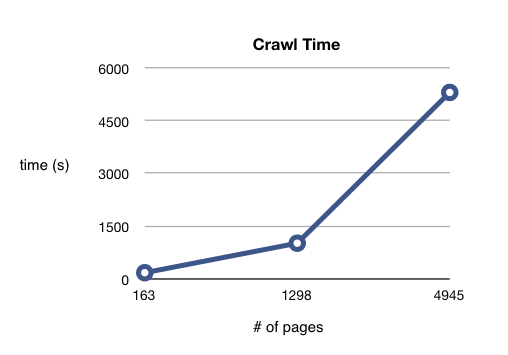
\includegraphics[scale=0.7]{images/crawl_performance.png}    
    \end{center}
    \caption{Performance Graph of Project Norris' Crawler.}
    \label{fig:performance}
\end{figure}

Scalability was an important design issue when designing and building Project Norris.  The following is a performance analysis of the attacking component, which can scale up.

\begin{center}
    \begin{table}
        \caption{Attacker Performance}
        \begin{center}
            \begin{tabular}{ | l | c | c | c | }
                \hline
                \# Pages & Total Crawl Time (s) & \# Attacking Components & Total Attack Time (s)  \\ \hline
                162 & 175 & 1 & 52 \\ \hline
                1294 & 811 & 1 & 101 \\ \hline
                4945 & 5911 & 1 & 325 \\ \hline
                161 & 213 & 3 & 47 \\ \hline
                1294 & 1655 & 3 & 59 \\ \hline
                4945 & 4643 & 3 & 134 \\
                \hline
            \end{tabular}
        \end{center}
        \label{table:scalability}
    \end{table}
\end{center}

As can be seen, in Table ~\ref{table:scalability}, when launching more instances of the attacking component, the total time taken to perform the attacks decreases.  However, this isn't the best representation of the scalability of the application.  In fact, the application is more suited to performing multiple vulnerability analysis runs, by launching multiple instances of the crawling component, as well as the attacking component.  

This is because there are likely to be more concurrent jobs for the attacking components by performing multiple scans, rather than from scanning one site and running multiple attacking components.  Crawling one site, large or small, will not necessarily result in a large succession of jobs for the attacker being generated, and the extra attacking components may be sitting idle, and therefore not demonstrating the scalability of the system.

Figure \ref{fig:performance2} shows the scalability data in an easier to digest manner.

\begin{figure}[!ht]
    \begin{center}
        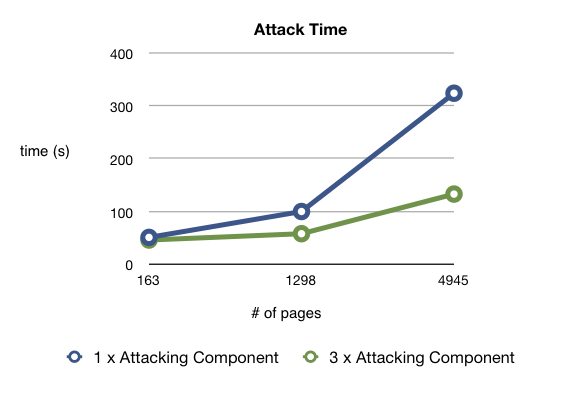
\includegraphics[scale=0.7]{images/attack_performance.png}    
    \end{center}
    \caption{Performance Graph of Project Norris' Attacker.}
    \label{fig:performance2}
\end{figure}
% TODO insert analysis

\section{Conclusions}

Current web application vulnerability detection techniques mostly involve static code analysis and, generally, this is limited to applications written in the PHP language.

Norris can be used to find vulnerabilities in web applications written in any language; it is a black box vulnerability scanner. 

Due to the designed architecture, Norris reports vulnerabilities as soon as it finds them, meaning it can be effectively used with web applications of any size.

It is an effective aide in the hunt for web application vulnerabilities and can crawl, parse and attack a website far quicker than a manual scan can.

\bibliography{webappsec}

\end{document}